\documentclass{article}
\usepackage[margin=1in]{geometry}
\usepackage{array}
\usepackage{longtable}
\usepackage{booktabs}
\usepackage{graphicx}
\usepackage{float}
\begin{document}
\footnotesize
\setlength{\tabcolsep}{4pt}
\renewcommand{\arraystretch}{0.9}
\section*{S7.3a Body}

\section*{S7.3(A)}
\begin{figure}[H]
\centering
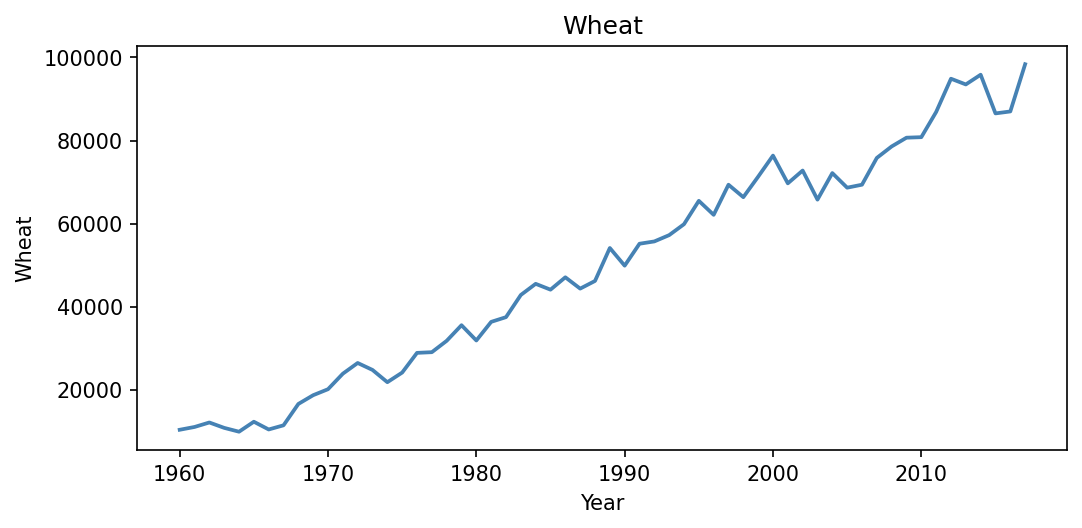
\includegraphics[width=0.95\linewidth]{S7.3A_wheat_ts.png}
\caption{Time-series plot of wheat}
\end{figure}
\begin{figure}[H]
\centering
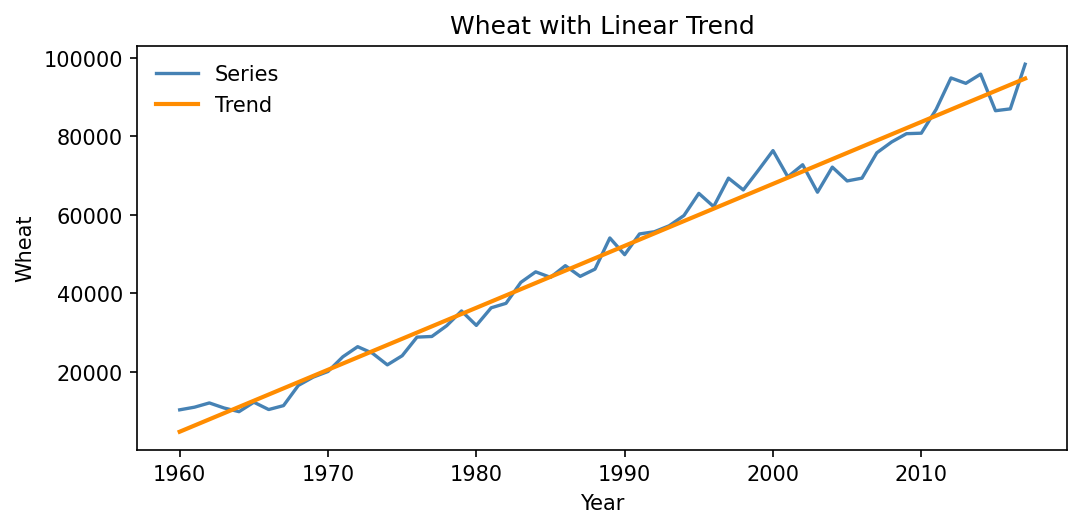
\includegraphics[width=0.95\linewidth]{S7.3A_wheat_trend.png}
\caption{Wheat with a quadratic deterministic trend}
\end{figure}
The series shows a strong upward deterministic trend. A linear trend in time fits nearly as well as a quadratic one; AIC/BIC slightly favor the linear specification. A log-linear trend is also plausible if growth is proportional. Economically, the trend is consistent with technological improvements (Green Revolution), expanded irrigation, fertilizer use, improved seed varieties, and policy support that raised yields and production over time.
(exponential growth) or a quadratic trend in time; the quadratic captures visible curvature in levels. 
Economically, the trend is consistent with technological improvements (Green Revolution), expanded irrigation, 
fertilizer use, improved seed varieties, and policy support that raised yields and production over time.
\begin{table}[H]
\centering
\begin{tabular}{lrrrr}
\hline
Method & RMSE & AIC & BIC & $n$ \\
\hline
linear & 3756.459 & 1123.420 & 1127.541 & 58 \\
quadratic & 3744.537 & 1125.051 & 1131.232 & 58 \\
cubic & 3744.701 & 1125.056 & 1131.237 & 58 \\
log-linear & 10548.084 & -17.531 & -13.411 & 58 \\
log-quadratic & 4225.527 & -95.285 & -89.103 & 58 \\
hp & 3516.936 &  &  & 58 \\
moving\_average & 2345.683 &  &  & 58 \\
lowess & 3217.104 &  &  & 58 \\
\hline
\end{tabular}
\caption{Trend fit summary for wheat}
\end{table}

\clearpage
\section*{S7.3b Body}

\section*{S7.3(B)}
\begin{figure}[H]
\centering
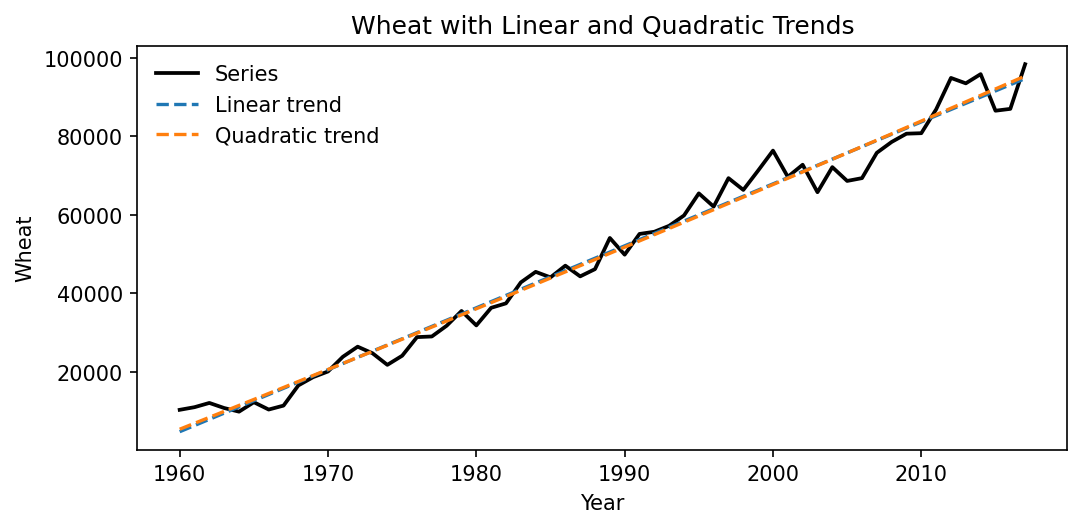
\includegraphics[width=0.95\linewidth]{S7.3B_wheat_trends.png}
\caption{Wheat series with linear and quadratic trend fits (dashed)}
\end{figure}
AIC: linear=1123.420, quadratic=1125.051; BIC: linear=1127.541, quadratic=1131.232. 
AIC and BIC both prefer the linear trend. This makes intuitive sense because the quadratic term is small and 
adds little visible curvature; information criteria penalize the extra parameter when the fit gain is minimal.

\clearpage
\section*{S7.3c Body}

\section*{S7.3(C)}
Using the AIC-preferred linear trend, the 2018 forecast for wheat production is 
$\hat{y}_{2018} = 96309.4$ with a 95\% confidence interval 
[94272.0, 98346.9]. 
This forecast assumes the deterministic trend is correctly specified, the error term is mean-zero with constant variance, 
and there are no structural breaks or policy/technology shocks between the sample and 2018.

\clearpage
\section*{S7.3d Body}

\section*{S7.3(D)}
\begin{figure}[H]
\centering
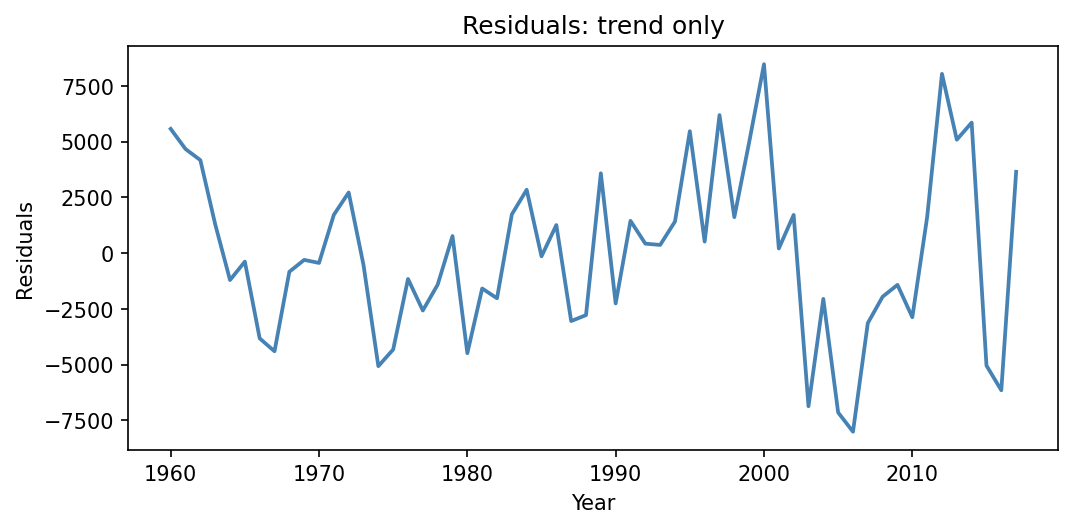
\includegraphics[width=0.95\linewidth]{S7.3D_resid_trend_only.png}
\caption{Residuals from trend-only model}
\end{figure}
\begin{figure}[H]
\centering
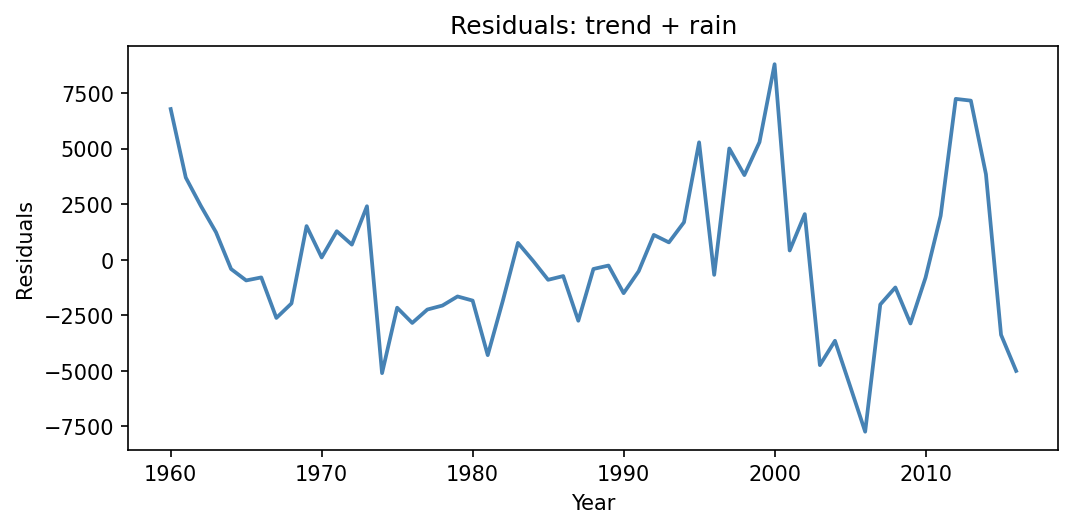
\includegraphics[width=0.95\linewidth]{S7.3D_resid_trend_rain.png}
\caption{Residuals from trend + rain model}
\end{figure}
\begin{figure}[H]
\centering
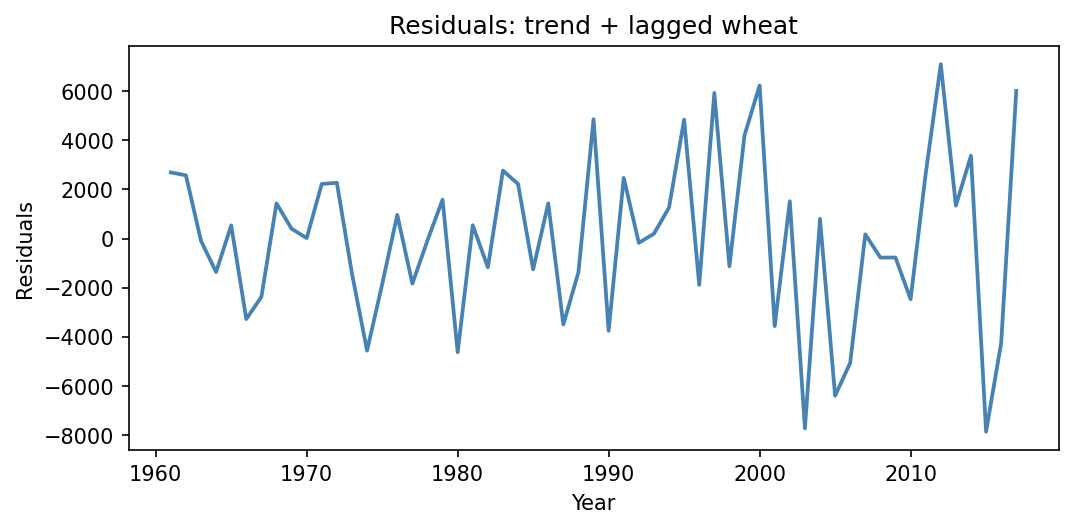
\includegraphics[width=0.95\linewidth]{S7.3D_resid_trend_lag_only.png}
\caption{Residuals from trend + lagged wheat model}
\end{figure}
\begin{figure}[H]
\centering
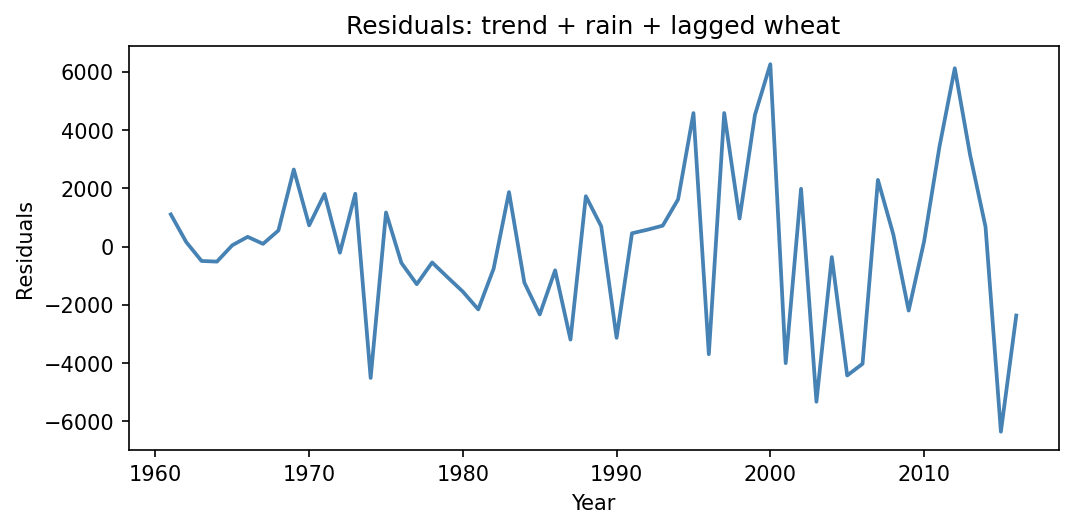
\includegraphics[width=0.95\linewidth]{S7.3D_resid_trend_rain_lag.png}
\caption{Residuals from trend + rain + lagged wheat model}
\end{figure}
Trend-only: $DW=1.093$; Ljung--Box $Q(4)=16.136$ ($p=0.003$). 
Trend + rain: $DW=0.766$; Ljung--Box $Q(4)=27.315$ ($p=0.000$). 
Trend + lagged wheat: $DW=2.035$; Ljung--Box $Q(4)=2.738$ ($p=0.603$). 
Trend + rain + lagged wheat: $DW=1.840$; Ljung--Box $Q(4)=3.665$ ($p=0.453$). 
Interpretation: adding lagged wheat substantially reduces serial correlation relative to trend-only or trend+rain, 
suggesting persistence in output that is not explained by rainfall alone. Rain may help explain levels but does not 
eliminate autocorrelation without a dynamic term.

\clearpage
\section*{S7.3e Body}

\section*{S7.3(E)}
We augment the trend model with rainfall to see whether it reduces residual dependence. 
Lag selection for Granger tests uses AIC with maxlags=4; selected lag = 1.

\begin{table}[H]
\centering
\begin{tabular}{llrrrrl}
\hline
Series & Test & Stat & $p$ & df & Dist & Reject \\
\hline
wheat (level) & ADF & 0.216 & 0.973 & 4 & ADF & No \\
wheat (level) & KPSS & 1.249 & 0.010 & 4 & KPSS & Yes \\
wheat (level) & PP & 0.934 & 0.994 & 11 & PP & No \\
wheat (diff) & ADF & -5.541 & 0.000 & 3 & ADF & Yes \\
wheat (diff) & KPSS & 0.106 & 0.100 & 5 & KPSS & No \\
wheat (diff) & PP & -13.712 & 0.000 & 11 & PP & Yes \\
rain (level) & ADF & 0.115 & 0.967 & 7 & ADF & No \\
rain (level) & KPSS & 0.981 & 0.010 & 3 & KPSS & Yes \\
rain (level) & PP & -8.703 & 0.000 & 11 & PP & Yes \\
rain (diff) & ADF & -3.199 & 0.020 & 8 & ADF & Yes \\
rain (diff) & KPSS & 0.167 & 0.100 & 15 & KPSS & No \\
rain (diff) & PP & -37.913 & 0.000 & 11 & PP & Yes \\
\hline
\end{tabular}
\caption{Stationarity tests for wheat and rain in levels and first differences}
\end{table}

\begin{table}[H]
\centering
\begin{tabular}{lrrrrl}
\hline
Test & Stat & $p$ & df & Dist & Reject \\
\hline
Granger: rain $\rightarrow$ wheat & 16.010 & 0.000 & 1, 53 & F & Yes \\
Granger: wheat $\rightarrow$ rain & 21.956 & 0.000 & 1, 53 & F & Yes \\
Lead exogeneity (rain) & 0.129 & 0.721 & 1, 50 & F & No \\
\hline
\end{tabular}
\caption{Exogeneity and Granger causality tests}
\end{table}

Trend + rain model residual diagnostics: $DW=0.766$; Ljung--Box $Q(4)=27.315$ with $p=0.000$. 
If residual serial correlation persists, the inference and forecast intervals from (c) are understated; 
a dynamic specification (e.g., AR errors, adding lagged wheat, or differencing) would be more appropriate.

\end{document}